
\chapter{C Pointers}
\label{chap:c-pointers}

 
\section{Introduction}
\label{sec:introduction-7}

Dynamically memory allocation is expensive. When to dynamically allocate a memory
\begin{enumerate}
  \item If the size is unknown at compile time
  \item If you want to use the data as long as you want, until you free/delete
  it
  \item The data will be created in heap (not in stack), i.e. which allows the
  object to be accessed from outside the scope where it's created.
\end{enumerate}

\subsection{Variable}
\label{sec:variable}

In any programming language, variables is a symbolic strings that help
you express your idea to the computers.  Indeed, you need to provide
two things, (1) the name and (2) the datatype.
\begin{lstlisting}
int i;
\end{lstlisting}
Given that two information, the compiler will reside a block in memory
big enough to hold the values (data) assigned to that variables. For
example, \verb!int! type needs 4 bytes, \verb!long! type needs 8
bytes. The size of a given type may vary on different machines or
different compilers.

In C, and some other language, we refer to the variable, say \verb!i!,
as ``object'' which is a named region of storage.

The physical memory of that variable is decided by the operating system.
However, C+ alows programmer to have the control of this memory location using 
the concept of pointers (Sect.\ref{sec:pointers-3}).



\subsection{Pointers}
\label{sec:pointers-3}


Pointers is a powerful feature of C programming language. 

A pointer is a variable that holds the address of a memory location as its
value.
To define a pointer variable that points to a memory block that holds the data
of type integer, we use
\begin{lstlisting}
//IMPORTANT: '*' goes with the name on the right-side ALWAYS

int* iptr; //RECOMMENDED - code clearer
           // than 
           // int *iptr; 
           // HOWEVER 
int *iptr, abc, *b; //RECOMMENDED - when we define both pointer and normal
                    // variable on the same line
\end{lstlisting}

A pointer is a datatype that can hold memory address of another variable of a
given type.
Whenever we define a variable of a given datatype (not pointer), the information
memory address of that variable is kept aside. Thus, when we assign a value to a
parameter the system will (1) find out the memory address, (2) put the data to
that memory address.


The value at the adress hold by the pointer, can be access using the unitary
operator \verb!*!, i.e. \verb!print, *iptr;! (print out the value at the
address which is the value of \verb!iptr!). To define a pointer that reference a
memory location whose data type can be anything (though still need to cast to a
proper data type when using it in the code), it uses a more powerful
feature called {\bf generic pointer} (Sect.\ref{sec:generic-pointer}).


The physical memory address of a variable can be retrieved using the ampersand
\verb!&!, i.e. the {\it unitary operator} \verb!&!. Example: \verb!&i! return
the memory address of $i$. As \verb!&! operator return the memory address
referencing to the object, we call it {\bf referencing operator}.

Example: what if we want to tell \verb!iptr! to hold the address of the integer
variable \verb!i!
\begin{lstlisting}
int *iptr;
int i = 10;

iptr = &i; // the same as *iptr = 10
print(&i) ;   // will print out 0x1000
\end{lstlisting}


{\bf More descussion}: If $i$ is associated with the memory location
0x1000 (hexadecimal). So, anytime we assign a value to $i$, this value
will be put to the memory location 0x1000.
\begin{lstlisting}
int i;
i = 10;
\end{lstlisting}
Of course, the memory address is determined by the system. We cannot
choose it. However, we can know the address once the system has
reserved the memory for the variable.


% In the previous example, $i$ hold the data value. What if we want to
% define a variable that only hold the memory location. The syntax to do
% this is 
% \begin{verbatim}
% type *variable;
% \end{verbatim}
% with \verb!type! is a particular datatype (intrinsic or
% derived). Then, we have the following example:
% \begin{lstlisting}
% int *iptr;
% int i;

% iptr = &i;
% \end{lstlisting}
% \verb!iptr! will hold the address of $i$. 

We now know that it's possible to access the memory address of a
variable using \verb!&! operator. The question is ``it is possible to
know the value at the memory location that a pointer's pointing
to?''. This can be done via the {\bf dereferencing operator} \verb!*!.

\begin{lstlisting}
int i = 10;
int *iptr=i;

print *iptr;  // return 10
\end{lstlisting}
It means that \verb!*iptr! is of type
\verb!int!. \textcolor{red}{That's why we write the start and the
pointer continuously. Remembering this convention in mind, it will
help you a lot later}. Pointer is also a legal datatype and the
variable is called {\bf address variable}, as it contains the address
of other variables. 

MORE COMPLICATED: 'abc' is a pointer pointed to a memory location whose value is
the memory address of some other memory location of type 'int'. So, 'abc' is a
pointer of type 'memory address'. How to declare this?
\begin{lstlisting}
int **abc;
\end{lstlisting}

{\bf Important}:
\begin{enumerate}
\item \verb!&! the ampersand goes with a variable (which in turn can
  be a pointer) $\rightarrow$ return the memory address of the
  variable ({\bf referencing operator}).
\item \verb!*! the asterisk goes with a pointer $\rightarrow$ return
  the value containing at this memory address
  ({\bf dereferencing operator}).
  
\begin{verbatim}
*ip++;
\end{verbatim}
The priority of asterisk (*) means that
\begin{verbatim}
(*ip)++; // the same as above
\end{verbatim}

\end{enumerate}

\subsection{Operation on pointer variable}

\begin{verbatim}
int n, *ip;		// int variable & int pointer declared
n = 5;			// initializes int variable
ip = &n;		// assigns address of n  to ip 
		// i.e. ip is now a reference to n

*ip = 7;	// dereferences ip
			// assigns new  value to memory ip points to (so: n = 7)

ip++;		// moves pointer to next location
			// caution!!! -- in this instance,
			// pointer now references unknown // location


/////////////////////
// unnamed dynamic variable

double *dp; 	// declares pointer
dp = new double; // allocates dynamic memory
delete dp; // releases dynamic variable

/////////////////////
// unnamed dynamic array

int size, *nums;
nums = new int [size]; // creates array

delete []nums; // releases dynamic array
\end{verbatim}

\subsection{pointer to pointer (T** arr) vs. reference to pointer (T*& arr)}
\label{sec:pointer-to-pointer}
\label{sec:reference-to-pointer}

\begin{lstlisting}
IEnumWbemClassObject*   pEnumerator;


 // PROS: as the reference cannot be a null-reference in a valid program. 
 // it guards against incorrect usage
HRESULT Query ( IN BSTR sQuery, OUT IEnumWbemClassObject* &pEnumerator ); // (1)

	--> we call
	hRes = Query ( sQuery, pEnumerator ); // (3)

HRESULT Query ( IN BSTR sQuery, OUT IEnumWbemClassObject** ppEnumerator ); // (2)

	
\end{lstlisting}


\subsection{Pointers vs. Arrays}
\label{sec:pointer-array}

\begin{verbatim}
/////////////////////
// unnamed dynamic array

int size, *nums;
nums = new int [size]; // creates array

//array name acts as pointer to first element
printf(*nums);   // == nums[0]
\end{verbatim}
 
Dynamic array elements can be referenced just like static array elements
\begin{verbatim}
// type is 'int' for this
nums[0], nums[1]

\end{verbatim} 


If $p$ is a cell [cell A] containing the index of (or address of, or pointer to)
another cell [cell B], then $*p$ refers to the content of the pointed-to cell
[i.e. cell B].

Pointers in BCPL are merely integer indices of the memory address. Example: If
$p$ contain the address of a cell, then $p+1$ is the address of the next cell.
So
\begin{verbatim}
*(V+i)
\end{verbatim}
means the $i$-th location after $V$. It's important to read
Sect.\ref{sec:c_pointer}.

Arrays in Algol 68 have either fixed bounds, or 'flexible:' to accommodate
flexible arrays. Pascal, originally, has only fixed-sized arrays and strings. 
C language treats strings as arrays of characters, terminated by a marker. Some
string operations are quite expensive as they have to search for the end of
a string. 

Passing to functions with pointer arguments derived from arrays are hard to
compile on vector machines, as it's hard to tell whether argument pointer
doesn't overlap data with any other argument pointer. 

Declaration syntax mimics Expression syntax.




\subsection{'far', 'near' and 'huge' pointer}

The using of these keywords are meaningful only on 16-bit Intel processors. So
it's considered obsolete nowadays. As far as virtual addresses is concerned, a
pointer has two components: a {\bf selector} (index to the base addresses of the
segment) and {\bf offset} (added to the base address to find the memory data).
\begin{enumerate}
  \item  When using \verb!near! pointer, it doesn't need a
'selector', i.e. implied selector. 
  \item When using \verb!far! pointer, it need explicit selector. However, when
  using pointer arithmetic on them, the selector DOESN'T change.
  \item When using \verb!huge! pointer, it need explicit selector. However, when
  using pointer arithmetic on them, the selector CAN change.
\end{enumerate}
\url{http://www.codeproject.com/Questions/103114/near-vs-far-vs-huge-pointers}

References:
\begin{enumerate}
  \item \url{http://cm.bell-labs.com/cm/cs/who/dmr/chist.html}
\end{enumerate}


\section{Generic pointer (void *)}
\label{sec:generic-pointer}

The next question is ``is there a way to define a pointer that can
point to anything (any datatype)?''. This can be done if the pointer
is defined using \verb!void! type. 
\begin{lstlisting}
void *ptr;
\end{lstlisting}
This is a {\bf generic pointer} and it is large enough to safely hold
a pointer to any type of object. 

As there is no variable of type \verb!void!, the pointer will not point to any
data and thus cannot be de-referenced. So, \textcolor{red}{it's important that
it needed to be casted to another kind of pointer first}. We can cast a generic
pointer to a pointer of a particular type without loosing any information.

Assign a generic pointer to a pointer of a particular type need
casting, tell the compiler that the value contained by this pointer
(i.e. \verb!&aptr!) is of type 'pointer to integer' (i.e. \verb!(int*)!) 
\begin{lstlisting}
int *iptr;
void *aptr;

iptr = (int*) &aptr;
\end{lstlisting}

Assign to generic pointers is okay.
\begin{verbatim}
void * ptr1, ptr2;
int b;

ptr1 = &b;

ptr2 = ptr1; //OKAY
ptr2 = (void*) ptr1; // OKAY
\end{verbatim}

However, assign a pointer to a generic pointer doesn't need type cast
\begin{lstlisting}
int *iptr;
void *aptr;

aptr = iptr;
\end{lstlisting}

\begin{framed}
Generic pointer cannot be dereferenced as well as being in any
arithmetic operation. We need to type cast it first to a particular
type. 
\begin{verbatim}
void * ptr;
int a,b;
a = 10;
ptr = &a;

// WRONG
b = *ptr + 10;

// CORRECT
b = * (int*)ptr + 10;
\end{verbatim}
\end{framed}


\section{NULL pointer: nullptr}
\label{sec:null-pointer}
\label{sec:nullptr}

NULL pointer is a special pointer, it does not hold a memory
address. So, dereferencing is illegal with NULL pointer. NULL is a
special constant defined in \verb!<stddef.h>! file. By default, assigning a
pointer to 0 is equivalent to NULL.

When you define a global or {\bf static} pointer, they are
automatically initialized to zero (NULL).
\begin{lstlisting}
static int *iptr;
\end{lstlisting}

Local pointer variables, like any other kind of variables, are not
automatically initialized. An {\it uninitialized} may receive any
random value. Thus, \textcolor{red}{SAFE PROGRAMMING}, when you first
define a pointer, you normally assign it to NULL (or 0).
\begin{lstlisting}
int *iptr=0;

int *iptr=NULL;
\end{lstlisting}

In C, NULL can be defined in one of these header files: \verb!stddef.h!,
stdlib.h, stdio.h, locale.h, string.h, time.h (in C99 it has wchar.h). In C++,
the equivalent header files are \verb!<cstddef>!, \ldots. Even though 0 and NULL
are the same. It is suggested not to use 0 as the semantics of NULL is more
expressive. 

In C++11, the value \verb!nullptr! (header file <cstddef>) should be used, and also there is a new type
\verb!nullptr_t!.
\url{http://stackoverflow.com/questions/924664/why-is-null-undeclared}


\section{Pointer constant vs. Constant pointer}
\label{sec:constant-pointer}

Just like defining an integer constant, or real constant, you can also define a
{\bf pointer constant}, i.e. the object that the pointer pointing to is
read-only.
\begin{lstlisting}
const int *iptr; // or
int const *iptr;
\end{lstlisting}
A pointer constant can point to any memory address of that type;
however we cannot modify the value storing in that memory
address. This is a convenient way to traverse an array (e.g. passing to
function's argument), without creating a duplicated copy, yet the array data
cannot be modified.

Another concept is {\bf constant pointer}, i.e. the memory address that this
pointer 'hold' cannot be changed, i.e. pointing to a fixed memory address; but
the value in that memory address can be changed. The syntax is strange
\begin{lstlisting}
int *const endptr = ptr + max;
\end{lstlisting}
As we cannot change the pointed memory address, we must assign it when
we define the constant pointer. Different from pointer constant, we
can modify the content at the memory location that the pointer
constant's pointing to.

MORE COMPLICATED: We can also define a pointer that point to a fixed
memory location whose content cannot change.
\begin{lstlisting}
const int a = 10;

const int *const endptr = a;
\end{lstlisting}
Here, we neither modify $endptr$ nor the value it points to, $a$. This
happens most frequently when we pass an array to a function that use
pointer to traverse the array but not allowed to modify any array
elements.

\section{typedef's of pointers}
\label{sec:typedef_pointers}

It's recommended NOT to use typedef to pointers. Review how \verb!const! is used
(Sect.\ref{sec:const_keywords}). The following example may cause confusing

\begin{verbatim}
typedef int* IntPtr;
const IntPtr p1;   // which means
         // const int * p1;

// but if we use
IntPtr const p1; // it would mean totally different
        // int * const p1;         
\end{verbatim}

\section{'restrict' pointer}
\label{sec:pointer_restrict}

Since C99, \verb!restrict! keyword was added to use with pointer declaration.
It's first important to understand about {\it strict-aliasing}
(Sect.\ref{sec:aliasing_rules}). The goal of using \verb!restrict! keyword is to
improve optimization for pointers that we know for sure that are not aliased,
i.e. not pointing to the overlapped memory location.

For example: we want to tell the compiler that the two pointers to type
\verb!int! passing to this function will never be pointing to the same place.
\begin{verbatim}
void foo(int * restrict i1, int * restrict i2);
\end{verbatim}


%%% Local Variables: 
%%% mode: latex
%%% TeX-master: "fortran_manual"
%%% End: 
\section{Pointers as function arguments}
\label{sec:pointers-as-function}

In C, function parameters are passed by value. So, any change inside
the function won't take effect after the function exit. 
\begin{lstlisting}
int i = 10;
print (i); // 10
incr(i);    // input the data value
print (i) ; // 10

    :
void incr(int j) { // j will hold a copy of the value
      // of the input parameter
 j = j + 1
}
\end{lstlisting}

To permanently change the value of a variable after calling the function, you
need to give it the parameter's address;
\begin{lstlisting}
void incr(int *iptr) // iptr will hold the address of 
        // the input parameter
{
   *iptr = *iptr + 1;
}
\end{lstlisting}
and inside the function, we need to {\it dereference} that to get access the
data value, as well as update the new value. To pass the memory address of a
variable, use \verb!&! operator. To dereference a pointer, we use \verb!*! operator.

\begin{lstlisting}
int i = 10;
incr(&i);  //input the address

    :
\end{lstlisting}


% \section{n-dimension pointer}
\section{Pointer vs. Array}
\label{sec:pointer_array}
\label{sec:array-and-pointer}

The keyword \verb![]! is used to denote an id-descriptor representing an array.
\begin{verbatim}
int a[10];  // it means that you're declaring 
           // 'a' is a pointer, pointing to the first element in the array
\end{verbatim}
So, \verb!a! is exactly the same as \verb!&a[0]!. Importantly, \verb!a! is a
constant pointer, i.e. we cannot change the location \verb!a! points at.


% Example:
% \begin{verbatim}
% void foo(char x[]);
%   // is the same as
% void foo(char* x);
% \end{verbatim}
% 
\textcolor{red}{\bf IMPORTANT}:
\begin{enumerate}
  
    \item an array is a constant pointer to the first element in the array, and
    thus, (unlike \verb!j! in the below example) we cannot make \verb!a!
    pointing to a different memory location
\begin{verbatim}
int a[3]; 
  // then a == &a[0]
  // or   *a == a[0]

   // or C++ way   
const int* array = new int[3]; 
\end{verbatim}    

    \item we can define a pointer to an array
    (Sect.\ref{sec:pointer-to-an-array}) which means \verb!j! is not a constant
    pointer, and thus we can make \verb!j! to point to a different memory location

\begin{verbatim}
int array[3];
   // the same as
int (*j)[3]; // j is a pointer to an array of 3 elements
j = (int(*)[3]) malloc(3);

\end{verbatim}
 
    \item the \verb![]! operator is a dereference operator with a shift
\begin{verbatim}
array[2]  
          is equivalent to 
*(array+2)       //depending upon the type of memory that the constant pointer 'array'
            // pointer to, it means we shift 2 'bytes' or 2 '4bytes' or 2 '2bytes' or 2 ...
\end{verbatim}
Adding a value X to an address of type T is equivalent to shifting that adddress
by \verb!X*sizeof(T)!.

Array element x[y] is interpreted as: start with the pointer x,
step y elements forward after the location pointed by the pointer x, and then
take whatever is there. 
\textcolor{red}{x[y] can also be written as *(x+y)}.


\end{enumerate}

Because of that, in most cases, array names are converted to pointers, e.g.
passing an array to function (Sect.\ref{sec:function_pass-array}).

Exceptions when array names is not converted to pointer
\begin{enumerate}
  \item  is when we use \verb!sizeof()! operator on an array, \label{sec:sizeof} 
  
\begin{verbatim}
int a[10];
int j = sizeof(a) ; // returns 10
\end{verbatim}
  which returns the  size (in bytes) of the array, not the size of the pointer. 
  
  The size of the array (in bytes) is equal the number of elements times the size of each
  element. So, it depends on the number of elements and the type of the
  elements.

NOTE: \verb!sizeof(pointer)! always return the same value, i.e. how many
bytes to store the address, regardless the number of elements the pointer
address or the type of those elements.

  \item an array cannot have zero length, i.e. no NULL array, but a pointer is
  okay, i.e. there is NULL pointer. Dereferencing a pointer to the first element
  in the array always return a valid result.
  
   
  \item is when \verb!&! operator is used. With an array
  
\begin{verbatim}
int array[7];
\end{verbatim}  
then, \verb!&array! is a pointer of type \verb!int(*)[7]! (i.e. to an array of 7
elements), not a pointer of type \verb!int*! (i.e. to a single value).
  
  \item we can do pointer arithmetic with pointers, but not with arrays. To do
  pointer arithmetic with an array, we need to do it via a pointer pointing to
  the address of the first element
\begin{verbatim}
char x[] = "abcdefghijklmnopqrstuvwxyz";
char* y = x; // now we can do pointer arithmatic with y

y++ ; //okay
x++ ; //error, as x is a constant pointer 
\end{verbatim} 
\end{enumerate}


Example: \verb!a! is an array that contains space for 8
integers
\begin{verbatim}
int a[8];
  // assign a value to an array offset
a[4] = 5;
\end{verbatim}

A pointer, however, doesn't contain space for any integer, but it can point to a
space for an integer. 
\begin{verbatim}
int *p;
 
p = &a[0]; // p holds the address of the memory that hold the value of a[0]

   // what can be confusing is we can write this way
p = a; 
   // and then we can use the pointer in the same way as in array
p[4] = 5;
\end{verbatim}


\section{Pointer in 1D arrays}
\label{sec:pointer-1Darrays}

In C, pointers and array names are interwined, but it is important to understand
the difference (Sect.\ref{sec:pointer_array}).
\begin{lstlisting}
int t[5];

t[i] = 4; // the same as *(t+i) = 4;
\end{lstlisting}
As \verb!t! is a pointer, which point to the first element (zero
index), thus \verb!t! is the same as \verb!&t[0]!.

We can also declare an pointer whose value is the memory address of an object of
type 'integer array of 5 elements'.
\begin{lstlisting}
int *ptr_t[5];

ptr_t+i = 4
\end{lstlisting}

{\bf NOTE}: Some books states incorrectly that an array name is a
{\bf constant pointer}.

\begin{lstlisting}
int my_array[] = {1,23,17,4,-5,100}; 
\end{lstlisting}
There are different ways to traverse through this array

\begin{enumerate}
\item array indexing
\begin{lstlisting}
for (i = 0; i < 6; i++)
{
  printf("my_array[%d] = %d  ", i, my_array[i]);   
}
return 0;
\end{lstlisting}
\item pointer
\begin{lstlisting}
for (i = 0; i < 6; i++)
{
  printf("ptr + %d = %d",i, *(ptr + i));        /*<-- B */
}
return 0;
\end{lstlisting}

{\bf NOTE}: doing \verb!ptr+1! or \verb!ptr++! or \verb!++ptr! will
increase the memory address that the pointer \verb!ptr! contains by an
amount of \verb!sizeof(type)! with \verb!type! in this case is
\verb!int!. 
\end{enumerate}

\section{Pointer in 2D arrays}
\label{sec:pointer-2Darrays}

There is no such multi-dimensional array data type in C. It facts, it's is an
array of (pointers to data elements) for 2D, or an array of (pointers to
(pointers to data elements)) in 3D.

\subsection{C}


In C, a multi-dimensional array is actuall 'an array of arrays'
(Sect.\ref{sec:C_array_2D}) 
\begin{lstlisting}
int arr[2][4]; // arr is an array of 2 elements, 
              //each element is an array of 4 elements

arr = [[1, 2, 3, 4], [5, 6, 7, 8]];
\end{lstlisting}
So 'arr' is an array of 2 elements, each element is an array of 4-element. Thus,
we can 
\begin{verbatim}
arr[0]  is equivalent to arr[0][0]

arr[1]  is equivalent to arr[1][0]
\end{verbatim}

NOTE:
\begin{verbatim}
        int a[2][3]
+----+----+----+----+----+----+
|    |    |    |    |    |    |
+----+----+----+----+----+----+
\_____________/
       |
       |    
       |
       p    int (*p)[3]
\end{verbatim}

If we declare
\begin{lstlisting}
int *p = arr; //p is a pointer of type 'int*' and point to the value '1'

int *p[4] = &(arr[0]);
int *p[4] = arr; //p is a pointer of type 'int*[4]' and point to
             // the first element of 2-element array arr
             
int *p[4] = &(arr[1]); //p is a pointer of type 'int*[4]' and point to
            // the second element of 2-element array arr             
            
int *p[2][4] = &arr; //p is a pointer of type 'int*[2][4] and 
          //point to the 2-element array arr            
\end{lstlisting}

To allocate a 2D array, i.e. an array of arrays, we use pointer-to-pointer.
Here, the array may not be contiguous, since you're allocating each row
separately
\begin{lstlisting}
#include <stdlib.h>
...
T **arr; // for any type T
arr = malloc(sizeof *arr * ROWS);
if (arr)
{
  size_t i;
  for (i = 0; i < ROWS; i++)
  {
    arr[i] = malloc(sizeof *arr[i] * COLS);
    if (arr[i])
      // initialize arr[i]
    else
      // panic
  }
}
\end{lstlisting}

To allocate array of arrays with contiguous memory, we do, e.g. \verb!char! type  
\begin{lstlisting}
char** allocate2Dchar(int count_x, int count_y) {
    int i;

    # allocate space for actual data
    char *data = malloc(sizeof(char) * count_x * count_y);

    # create array or pointers to first elem in each 2D row
    char **ptr_array = malloc(sizeof(char*) * count_x);
    for (i = 0; i < count_x; i++) {
        ptr_array[i] = data + (i*count_y);
    }
    return ptr_array;
}
\end{lstlisting}
For deallocation, a normal \verb!free()! on \verb!ptr_array! is NOT enough, as
we have two pointers \verb!char* data! (which is actually \verb!char*!
\verb!ptr_array[0]!, \verb!char**ptr_array! so we use
\begin{lstlisting}
/* free data array first, then pointer to rows */
void free2Dchar(char** ptr_array) {
    if (!ptr_array) return;
    if (ptr_array[0]) free(ptr_array[0]);
    free(ptr_array);
}
\end{lstlisting}

\subsection{C++}

In C++, it's recommended to use \verb!boost::multiarray!. 
\begin{lstlisting}
int main()
{
   int  x;
   int  y;
   getWidthAndHeight(x,y);

   // declare a 2D array of int*
   boost::multi_array<int*,2>   data1(boost::extents[x][y]);

   data[2][3] = new int(6);
}
\end{lstlisting}
Otherwise, in C++, an
array of [rows][cols], we do
\begin{lstlisting}
// Create 2D array of pointers:
int*** array2d = new (int**)[rows];
for (int i = 0; i < rows; ++i) {
  array2d[i] = new (int*)[cols];
}

// Null out the pointers contained in the array:
for (int i = 0; i < rows; ++i) {
  for (int j = 0; j < cols; ++j) {
    array2d[i][j] = NULL;
  }
}
\end{lstlisting}

References:
\begin{enumerate}
  \item \url{http://stackoverflow.com/questions/8617466/a-pointer-to-2d-array}
  \item
  \url{http://stackoverflow.com/questions/5040496/how-can-i-allocate-a-2d-array-using-double-pointers}
\end{enumerate}

\subsection{C++11}

It uses \verb!std::array!.

\url{http://cpptruths.blogspot.com/2011/10/multi-dimensional-arrays-in-c11.html}

\subsection{Jagged array}

\begin{lstlisting}
int main()
{
    std::vector<std::vector<int*> >   data1;

    data1.push_back(std::vector<int*>(10,NULL));
    data1[0][3] = new int(7);
}
\end{lstlisting}

\section{Pointers in strings}
\label{sec:pointers-strings}

In C, a string is an array of characters terminated by a
{\bf null character}. Be aware that this is different from NULL
pointer (in uppercase). The null character is an escape zero
\verb!`\0'!, which is one byte; while NULL is the name of the macro
used to initialize a null pointer. 

Thus, like an array, a string variable is also a pointer pointing to
the first character in the array.
\begin{lstlisting}
char *str;
char str[10];
\end{lstlisting}

There are different way to define a string
\begin{enumerate}
\item listing
\begin{lstlisting}
my_string[0] = 'T';
    my_string[1] = 'e';
    my_string[2] = 'd':
    my_string[3] = ' ';

\end{lstlisting}

\item set
\begin{lstlisting}
char my_string[40] = {'T', 'e', 'd', ' ',};
\end{lstlisting}
\item better way
\begin{lstlisting}
char my_string[40] = "Ted";
\end{lstlisting}
Using double quotes, the null character is appended automatically.
\end{enumerate}

\section{Pointer-to-pointer (C language) vs. Reference-to-pointer (C++)}

Are there any advantages of one over the other? I am afraid, no. The usage of
one of both, for some programmers are just personal preferences.
If you find that the ptr-to-ptr and ref-to-ptr syntax are rather hard to
understand, you can just use the "return the pointer" method.
\begin{verbatim}
ClassA* func()
{
  ClassA* p = new ClassA();
  // do my things with p
  // ...
  return p;
}
\end{verbatim}



\subsection{Pointer to Pointers (C language)}
\label{sec:pointer-pointers}


Pointers is a data type that hold the memory address of a variable of
a given type. The question is ``what if the given type is also a
pointer'' as pointer is also a legal datatype. 

Example: \verb!ptr! is the pointer whose content is the address of an int value
\begin{verbatim}
             [300] -------> [...]
        ptr= 100             300

    [100] ---> [???] -------> [...]
pptr=20         100            ??? 
\end{verbatim}
\verb!pptr! is the pointer whose content is the address of a pointer.


The declaration of a pointer to a pointer is defined using \verb!**!
operator.
\begin{lstlisting}
int i = 5, j = 6; k = 7;
int *ip1 = &i, *ip2 = &j;

int **ipp = &ip1;
\end{lstlisting}

% \begin{lstlisting}
% int **ipp;
% int i = 5;
% 
% ipp = &i;
% \end{lstlisting}
 
\begin{figure}[hbt]
  \centerline{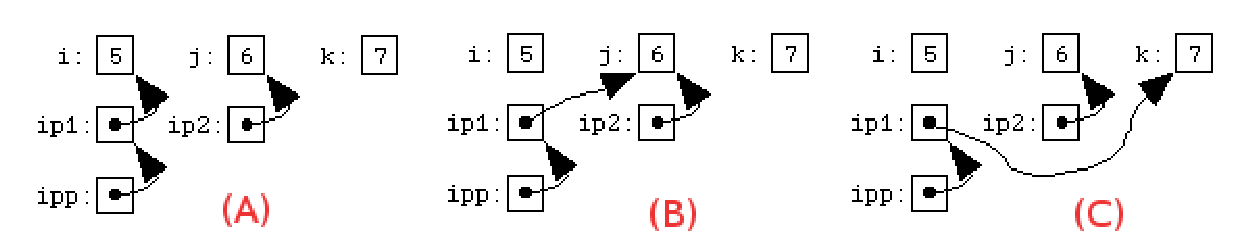
\includegraphics[height=2cm,
    angle=0]{./images/c_pointer.eps}}
\caption{(A) ; (B); (C); }
\label{fig:c-pointer}
\end{figure}

\begin{itemize}
\item [A] \verb!ipp! is the ptr-to-ptr, which hold the address of ip1.
\verb!*ipp! is the pointed pointer, \verb!**ipp! is the de-referenced twice variable. 

\begin{lstlisting}
ipp = &ip1;
\end{lstlisting}
\item [B] the content of the memory location that \verb!ipp!
  referencing to, which is the address of the memory location that
  \verb!ip1! is referencing to, change to the content of \verb!ip2!,
  which is the memory address that \verb!ip2! referencing to which
  hold the value of the variable $j$.
\begin{lstlisting}
*ipp = ip2;
\end{lstlisting}
\item [C] the content of the memory location that \verb!ipp!
  referencing to, which is the address of the memory location that
  \verb!ip1! is referencing to, change to the address of the memory
  holding the value for \verb!k!.
\begin{lstlisting}
*ipp = &k;
\end{lstlisting}
\end{itemize}


USAGE: This is widely used in C language as argument passing that allows the
function to modify the content value of the pointer
(Sect.\ref{sec:pointer-2Darrays}). In C++, it has passing by reference, so
passing a pointer to pointer is not the only option.

\begin{verbatim}
void func(int** ppInt)
{
  //Modify the pointer, ppInt points to
  *ppInt=&g_One;

  //You can also allocate memory, depending on your requirements
  *ppInt=new int;

  //Modify the variable, *ppInt points to
  **ppInt=3;
}
\end{verbatim}

% {\bf When to use pointers to pointers}:
% Let's see the simple example
% \begin{lstlisting}
% f(int *ip)
% {
%    *ip = 5;  // write to the location that ip points to the value 5
% }
% 
% ..........
% int i;
% f(&i);
% print (i);  // 5
% \end{lstlisting}
% It means that a function to return a value of type int, it used a
% parameter of type pointer-to-int.
% 
% Now, what if we want a function return a value of type pointer of
% string. 


\subsection{Reference to pointer (C++)}
\label{sec:reference-to-pointer}

Reference operator \verb!&! was added to C++98  (Sect.\ref{sec:&_operator})

\begin{verbatim}
//function prototype
void func(int*& rpInt);

int main()
{
  int nvar=2;
  int* pvar=&nvar;
  func(pvar);
  ....
  return 0;
}
\end{verbatim}

\url{http://www.codeproject.com/Articles/4894/Pointer-to-Pointer-and-Reference-to-Pointer}

\section{Dynamic memory allocation}
\label{sec:dynam-memory-alloc-1}

When working with pointers, it's important to know how to allocate memory
dynamically. You can dynamically allocate a region of memory and assign a
pointer to hold the memory address at which the newly created object resides.

Dynamic memory allocation is a very important part of most computer systems.
However, it can lead to memory leak if the dynamically allocated
memory is not freed properly at the end of the program.

\begin{enumerate}
  \item C98:  We will cover different ways to implement dynamic memory
  allocation in Sect.\ref{sec:understand_malloc}.

  \item C++ Boost library: Sect.\ref{sec:Boost::Pool}
\end{enumerate}

\subsection{Boost::Pool (C++)}
\label{sec:Boost::Pool}

Boost::Pool is often used when there is a lot of allocation and deallocation of
small objects.
\footnote{\url{http://www.boost.org/doc/libs/1_43_0/libs/pool/doc/index.html}}



\subsection{ANSI C: malloc() \& free()}
\label{sec:understand_malloc}

\begin{verbatim}
#include <stdlib.h>

void *malloc (size_t);
void free (void *);
void *calloc(size_t nmemb, size_t size);
void *realloc(void *ptr, size_t size);
void *reallocarray(void *ptr, size_t nmemb, size_t size);
       
\end{verbatim}
\url{http://man7.org/linux/man-pages/man3/malloc.3.html}


Early implementation of dynamic memory allocation was done by Doug Lea for C
language in 1987 as \verb!dlmalloc()! (dl means Doug Lea). This allocator
provides the basic implementation of the standard C routines: \verb!malloc(),
free(),! and \verb!realloc()!, as well as other auxiliary utility routines
\footnote{\url{http://gee.cs.oswego.edu/dl/html/malloc.html}}.
The dynamically allocated memory need to be free manually using \verb!free!
function. 

\textcolor{red}{Early malloc() is not thread-safe}: The \verb!malloc()!
allocates memory on a global heap (Sect.\ref{sec:heap_stack}), i.e. shared by
multiple threads, and it is possible that two different invocations of
\verb!malloc()! that happens at the same time, i.e. they can return the same
memory block when the second malloc call happen before the address of the chunk
is fetched, but the chunked is not marked as unavailable yet.

There is 3 main "versions" of C in ANSI C, C99 and C11
(Sect.\ref{sec:C11-intro}).
Since POSIX.1-2008 (Sect.\ref{sec:POSIX}), which is suported by C11,
\verb!malloc()! is thread-safe. Thread-safe implementation of \verb!malloc()!
uses a lock-based synchronization.
However, this still can cause deadlock when \verb!malloc()! is called from a
signal handler (Sect.\ref{sec:signal_handler}).

\begin{verbatim}
malloc();            //initial call
  lock(memory_lock); //acquire lock inside malloc implementation
signal_handler();    //interrupt and process signal
malloc();            //call malloc() inside signal handler
  lock(memory_lock); //try to acquire lock in malloc implementation
  // DEADLOCK!  We wait for release of memory_lock, but 
  // it won't be released because the original malloc call is interrupted
\end{verbatim}
So, the current implementation of \verb!malloc()! is thread-safe, but not
reentrant. None of the common versions of malloc allow you to reenter it (e.g.
from signal handler). 
\url{http://stackoverflow.com/questions/3941271/why-are-malloc-and-printf-said-as-non-reentrant}

To ensure signal handler safe:
\begin{enumerate}
  \item no dynamic memory allocation: avoid using malloc(), std::string,
  std::vector (which call malloc() internally)  
  
  \item  no buffered stdio or iostreams
\end{enumerate}

\subsection{C: malloc() or calloc()}
\label{sec:malloc()}
\label{sec:calloc()}

Allocating memory to be accessed by the CPU is most often accomplished using the
C standard library function malloc. If you have CUDA library, you can also
consider using cudaMallocHost() - Sect.\ref{sec:cudaMallocHost}.
 
We need to use the header file
\begin{enumerate}
  \item Linux: either  <stdlib.h> (in C) or <cstdlib> (in C++)
  \item Windows: <windows.h>
\end{enumerate}

\verb!calloc()! guarantees zero-initialize the buffers (clear-alloc) using
\verb!memset!, while \verb!malloc()! leaves the buffer uninitialized
(memory-alloc). 

As zeroing out the memory takes sometimes, if you want it fast, and zero-value
is not important, and you should consider using \verb!malloc()!.
The memory is allocated on heap (Sect.\ref{sec:heap_stack}).

IMPORTANT: The returned pointer is not a constant pointer, so we can change its
pointing address. However, we will no longer pass that pointer to the
\verb!free! function as it wont point to the first byte any more. So, it's
important to treat that pointer as a constant, i.e. don't change it.

\textcolor{red}{Another important but less known difference is that in some O/S
with optimistic memory allocations, e.g. Linux, the pointer returned by malloc()
is not backed by real memory until the program actually touches it. As calloc()
set the zero values, the O/S sure is backing the allocation with actual RAM or
swap}. So, calloc() is slow not only it set the values, but also it needs to
find a suitable memory area by possibly swapping out other processes.

A rather often-overlooked advantages of \verb!calloc()! is that it make sures
to avoid overflow
\begin{verbatim}
// overflow occurs if 'count' > SIZE_MAX/sizeof(*bar)
size_t count = get_int32(file);
struct foo *bar = malloc(count * sizeof *bar);
\end{verbatim}
\url{http://stackoverflow.com/questions/1538420/difference-between-malloc-and-calloc}


A generic pointer \verb!void*! pointing to the first byte of memory allocated is
returned, which can be mapped to any other poniter type.
\begin{lstlisting}
#include <stdlib.h>

double *dptr = malloc(n* sizeof(double));

if (dptr == NULL) printf("cannot allocate")
else free(dptr);
\end{lstlisting}

\verb!malloc! return a generic pointer to the first byte of the
allocated memory. Even though we assign a generic pointer to a double
pointer, we don't need to use type cast as in this case, it is
automatically managed by C compiler. However, you can also do it explicitly 

\begin{lstlisting}
double *dptr = (double *) malloc(n* sizeof(double));
if (dptr != 0) {
   /* success, do it */
?
\end{lstlisting}
If the task is failed (for some reason), it returns a NULL pointer. {\bf NOTE}:
\textcolor{red}{Always check the successfullness of }\verb!malloc!.

{\bf NOTE}: When allocating an array of zero element, \verb!malloc(0)!, the
result is implementation defined, which can be either a NULL pointer or an
address. We don't want it to return NULL for two reasons: (1) we want to use
NULL return as a sign that malloc() has failed, (2) we want a unique pointer for each
call to malloc() so that we can add it to the block table.
\begin{verbatim}
    void * ptr;
    ptr = malloc(0);
    free(ptr);
\end{verbatim}
To work arround, a suggested user-defined implementation to check for zero-size
and always allocate at least sizeof(void*). NOTE: Here we consider
MPI-application. However, using this can slow down the performance. That's why
we can define a macro \verb!FAST_MALLOC! to use when compiling the code.

{\small \begin{verbatim}
#ifdef FAST_MALLOC
  #define ddcMalloc(size)      malloc(size)
#lse


#define ddcMalloc(size) _ddcMalloc(size, __ddcLine(__FILE, __LINE))

void* _ddcMalloc(size_t size, char* location)
{
	if (size == 0) size=sizeof(void*);
	void *ptr = malloc(size);
	if (!ptr){
	  printf(``Mem-allocate failed on task %d (%zu bytes at %s)\n''
	         ``                        memUsed=%8.2f\n'', 
	         getRank(0), size, location, _memUd/b2mb)
	  printHeapInfo(stdout);
	}else{
	   int b = addBlock(ptr, size, location);
	}
	return ptr;
}}
\end{verbatim}}


{\bf calloc()}: The data allocated by \verb!malloc! is not guaranteed to be
initialized to any value. So, a variant is \verb!calloc! that automatically
initialize the data to zeros.

\begin{lstlisting}
type * pData;
pData = calloc(unsigned int num, size_t sizeof(type))
\end{lstlisting}

We can allocate memory for a structure
\begin{verbatim}
#include <stdlib.h>
#include <stdio.h>

typedef struct rec{
  int i;
  float PI;
  char A;
} RECORD;

struct rec2{
  int i;
  float PI;
  char A;
}

int main() {
  RECORD *ptr_one;
  ptr_one = (RECORD*) malloc(sizeof(RECORD));

  struct rec2 *ptr_two;
  ptr_two = (struct rec2 *) malloc(sizeof(struct rec2)); 
  ...

  printf ("First value %d\n", (*ptr_one).i);
  printf ("Second value %f\n", ptr_one->PI);  
  free(ptr_one);
  free(ptr_two);
  return 0; 
}
\end{verbatim}
NOTE: There are two ways to access a data element of a pointer. Most people use
\verb!->! operator.

NOTE: When allocating a string \verb!char*!, always add 1 to the expected string
length.
\begin{verbatim}
int strlen = 10;
char * str;

alloc(str, sizeof(*str) * (strlen+1));
\end{verbatim}

\subsection{C: realloc()}
\label{sec:realloc()}

\verb!realloc(ptr, size)!
\begin{verbatim}
void* realloc (void* ptr, size_t size)
\end{verbatim}
\begin{itemize}
  \item C90 (C++98): if the size is zero, then the memory previously allocated
  for \verb!ptr! is freed using \verb!free()! and a NULL pointer is returned.
  \item C99/C11 (C++11): depend on the particular library implementation, which
  can be either a NULL pointer, or a pointer to some other location that shall
  not be dereferenced.
\end{itemize}
Other situations:
\begin{enumerate}
  \item  If \verb!size! is not zero, and the function fails to allocate the requested
block of memory, a NULL pointer is returned, while the memory pointed by
\verb!ptr! is unchanged. If the function is success,  the function return a
pointer to the memory block allocated by the function.
  \item If the new size if bigger, the value of the newly allocated portion is
  indetermine.
  \item If \verb!ptr! is a NULL pointer, the behavior is like \verb!malloc()!.
\end{enumerate}

A suggested approach: it's best to store the return value in a temporary
variable. If \verb!realloc()! fails, e.g. not enough memory, then it returns
NULL, while the original pointers is NOT freed. So, it's better not to change
the address of the original before knowing what's really happening
\begin{verbatim}
char *tmp = realloc(result, newsize);
if (tmp == NULL)
{
    // handle error here and free the memory
    free(result);
}
else
{
    // reallocation was successful, re-assign the original pointer
    result = tmp;
}
\end{verbatim}

\subsection{C: xalloc()}
\label{sec:xalloc()}

\subsection{C: alloca() on stack}
\label{sec:alloca()}

For small-size array with unknown size at compile time, we can use
\verb!alloca()! to allocate the memory on stack (Sect.\ref{sec:heap_stack}).
Here, the memory is automatically freed when the calling function exit. So,
there is no need to call \verb!free()!.  This is often used with array
(Sect.\ref{sec:alloca}).


\subsection{C: free() and dangling pointer}
\label{sec:free()}

{\bf NOTE}: \verb!free()! only works with dynamically allocated pointers
(Sect.\ref{sec:dynam-memory-alloc-1}), not with global or static pointers.

When you have two pointers pointing to the same memory location, and you free
that memory allocation, the second pointer becomes a dangling pointer, i.e. a
pointer that point to an invalid memory.

\begin{verbatim}
char* ptr = malloc(100);
...
free(ptr);
ptr = NULL;
\end{verbatim}
Then, later on, if you accidently free a NULL pointer, the O/S silently does
nothing.

\subsection{using macros for debugging purpose}

ANSI C preprocessor will replace the special symbols \verb!__FILE__! and
\verb!__LINE__! with the file and line number of the macro's invocation

\begin{verbatim}
void *malloc (size_t);
void *_malloc_leap (const char *file, int line, size_t size);
#define malloc(size) _malloc_leap(__FILE__, __LINE__, size)

void free (void *);
void _free_leap (const char *file, int line, void *);
#define free(ptr) _free_leap (__FILE__, __LINE__, ptr);

\end{verbatim}



\section{Type cast}
\label{sec:type-cast}

Typecasting is the concept of converting the value of one type into another type
(type conversion). The conversion can be implicit (i.e. done automatically by
the compiler), or explicit (i.e. the target type is coded in by the programmer).

There are three types of explicit conversion.
\begin{enumerate}
  \item {\bf checked} : prechecked at runtime before the conversion. If the
  destination type cannot hold the source value, an error is raised. 
  
  \item {\bf unchecked}: no checked is performend. If the destination type
  cannot hold the source value, the result is {\it undefined}. 
  
  \item {\bf bit pattern}:  the data is not interpreted at all, i.e. the raw-bit
  representation of the source is copied, and then re-interpreted according to
  the new type. 
\end{enumerate}

The C/C++ type-cast is either ``unchecked'' or ``bit pattern''
\begin{itemize}

  \item C style - Sect.\ref{sec:type-cast-C}: \verb!(new_type)expression!

\begin{lstlisting}
class A;
class Asub: public A;

A* ptr = new Asub();

Asub& b = (Asub)ptr;

// or 
float fl = 5.4;
int ii = (int) fl; 
\end{lstlisting}  

  \item C++ style: It uses one of the following syntax
  
\begin{Verbatim}
new_type(expression)
    
dynamic_cast <new_type> (expression)
reinterpret_cast <new_type> (expression)
static_cast <new_type> (expression)
const_cast <new_type> (expression)
 \end{Verbatim}
\end{itemize}


\subsection{In C}
\label{sec:type-cast-C}

With implicit type-casting, typically, the compiler will issue a warning for
each implicit conversion it does. An example is 
\begin{verbatim}
int i_value   = 16777217;
float f_value = 16777216.0;
    
if (i_value > 2) i_value = f_value; /* implicit */    
\end{verbatim}

then the warning can be
\begin{verbatim}
conversion from 'double' to 'int', possible loss of data.
\end{verbatim}

Usually, the compiler do type cast promotion in the order for the intrinsic data
type
\begin{verbatim}
int -> unsigned int -> long -> unsigned long -> long long -> 
unsigned long long -> float -> double -> long double
\end{verbatim}

\subsection{--   (T)somevariable}

\textcolor{red}{However, it's considered a good programming practice to use
explicit type casting with {\bf cast operator}}, i.e.
the target type is wrapped inside the parantheses, \verb!(T)expression!.
\begin{verbatim}
some_type b;
type_name a;

a = (type_name) b;
\end{verbatim}


Example:
\begin{verbatim}
double da = 3.3;
double db = 3.3;
double dc = 3.4;
int result = (int)da + (int)db + (int)dc; //result == 9
\end{verbatim} 

One use for type cast is to use ASCII characters
\begin{verbatim}
    for ( int x = 0; x < 128; x++ ) {
        /* Note the use of the int version of x to output a number and the use
         * of (char) to typecast the x into a character which outputs the
         * ASCII character that corresponds to the current number
         */
        printf( "%d = %c\n", x, (char)x );
    }
    getchar();
\end{verbatim}

In C, the compiler doesn't detect errors like this. C-stype cast allows an INT
pointer to point to a CHAR pointer.
\begin{verbatim}
char c = 10;       // 1 byte
int *p = (int*)&c; // 4 bytes
\end{verbatim}

Writing to 4-byte pointer will either cause run-time error or overwrite adjacent
memory, as the compiler doesn't check for data type compatibility. 
\begin{verbatim}
*p = 5; /* potential error */
\end{verbatim}


\subsection{In C++}
\label{sec:type-cast-C++}

We can still use C-style in C++; yet it's suggested to use C++ style which
utilizes {\it explicit type conversion}. C++ provides 4 different ways of
type-cast
\begin{Verbatim}
new_type(expression)
    
dynamic_cast <new_type> (expression)
reinterpret_cast <new_type> (expression)
static_cast <new_type> (expression)
const_cast <new_type> (expression)
 \end{Verbatim}

NOTE:
\begin{Verbatim}
MyClass *m = (MyClass *)ptr;  // C-style
           = MyClass* (ptr); // C++-style

           = const_cast<MyClass *> ptr; 
           = static_cast<MyClass *>(ptr);  // recommended: C++-style 
           = static_cast<MyClass *> (const_cast<MyClass *>)ptr;
           
MyClass *m = reinterpret_cast<MyClass *> ptr;
           = reinterpret_cast<MyClass *> (const_cast<MyClass *>)ptr;
MyClass *m = dynamic_cast<MyClass *>(ptr); // C++-style
\end{Verbatim}

\subsection{-- T(somevariable)}

The C style \verb!(T)something! and the C++ style \verb!T(something)! are
equivalent for type cast and both should be avoided in C++; the latter one
(C-style) should be avoided more.  IMPORTANT: Using C++-style for a class
object, the downcast also strips off \verb!const!-property if the original
pointer is marked with \verb!const! attribute (to preserve this, use
\verb!static_cast! - Sect.\ref{sec:static_cast}).


In C++, with class (object-oriented) and inheritance, it's getting more
important to understand type-casting. There are two ways: downcasting and
upcasting.
\begin{itemize}
  \item Upcasting: convert a derived-class reference or pointer to a base-class.
  This allows us to treat the object of the derived-class as if it was of the
  base-class type. \textcolor{red}{This is always allowed for {\bf public}
  inheritance} (Sect.\ref{sec:inheritance_public}).  We are allowed to use
  implicit type-cast. Upcasting can cause \textcolor{red}{\it object slicing}
  when the object of derived-class is passed by value as a base-class object
  (Sect.\ref{sec:object-slicing}).
  
  \item Downcasting: convert a base-class reference or pointer to a
  derived-class. Explicit type-cast is required. 
\end{itemize}


A type-cast like this
\begin{verbatim}
T* ptr = (T*) var;
\end{verbatim}
doesn't tell right away, in C++, if 
\begin{enumerate}
  \item a cast is from a base class to a derived class or the other way around
  \item a cast stripes the constant object \verb!const! or not
  \item a cast is from an integral type to a pointer or not 
\end{enumerate}

To help making it clear and to improve safety, C++11 provides new syntax. The 4
new different typecast operators all use angle brackets \verb!< ... >! and put the target type inside
\begin{enumerate}
  \item \verb!static_cast!
  \item \verb!reinterpret_cast!
  \item \verb!const_cast!
  \item \verb!dynamic_cast!
\end{enumerate}
Using one the 4 above syntax, C++ style type cast are checked
by the compiler. Each cast handles one specific sort
of convention or a family of related conversions. This allows the compiler to go on
and check that you're not accidentally doing something that you are not
intended.


\subsection{-- static\_cast}
\label{sec:static_cast}

\verb!static_cast! is used for type-casting, while maintaining the
const-attribute. 

Example of the C-style cast problem: You have the code
\begin{verbatim}
void DoSomething(Base* ptr) {
    Derived* derived = (Derived *) (ptr);
    DoSomethingElse(derived);
}
\end{verbatim}
and now you don't want to make change to the content of the object pointed to
by \verb!ptr!, so you want to emphasize to mark the argument with \verb!const!
(see Sect.\ref{sec:const_its-position})

\begin{verbatim}
void DoSomething(Base const * ptr) {
    Derived* derived = (Derived *) (ptr);
    DoSomethingElse(derived);
}
\end{verbatim}

However, now it is the problem. Using C-style the downcast also strips off
\verb!const!-property. This is an easily bug if DoSomethingElse() method really
modify the input. If your code is
\begin{verbatim}
void DoSomething(Base const * ptr) {
    Derived* derived = static_cast<Derived *>(ptr);
    DoSomethingElse(derived);
}
\end{verbatim}
which keep the \verb!const!ness property of \verb!ptr! and pass to
\verb!derived!. Thus, the compiler error is raised if \verb!derived! is modified
inside DoSomethingElse().

\begin{mdframed}

In C++, \verb!static_cast<>()! does two things 
\begin{enumerate}
  \item casting to the new type while keeping the existing property of the
  original object (e.g. \verb!const!ness if possible), 
  
  \item make sure the type conversion is compatible. Thus, using
  \verb!static_cast<>! is a safer way as it gives compile time checking
  capability, which is not available in C (see above).  
\end{enumerate}

\end{mdframed}

\begin{verbatim}
char c = 10;
int *q = static_cast<int*>(&c); // compile-time error detection
\end{verbatim}

So, the compiler will check for type compatible. Also, using it is more
readable, and can spot easily inside a C++ code. It's widely used for conversion
from derived class to base class (i.e. inheritance
Sect.\ref{sec:OO_inheritance}). \textcolor{red}{This is the first cast you
should attempt to use, i.e. if we know that the pointer is actually pointing to
an object of a specific type}. 

IMPORTANT: It's possible to map \verb!const! objects to non-const objects
(Sect.\ref{sec:const_C++}): read \verb!const_cast<>!
(Sect.\ref{sec:const_cast}).

Example:
\begin{verbatim}
	enum my_numbers { a=10, c=100, e=1000 };

	const my_numbers b = static_cast<my_numbers> (50);
	const my_numbers d = static_cast<my_numbers> (500);
\end{verbatim}

\subsection{-- const\_cast}
\label{sec:const_cast}

In C++, if the original object being casted has \verb!const! property or
\verb!volatile! property, you can cast that propery away from the object, i.e.
assign to a pointer in that the memory can be modified via that pointer.
Because of this, it's recommended NOT to use \verb!const_cast<>! as it reveals
(most of the time) a flaw in the design, i.e. a not-supposed-to-be-modified
data now become modifiable-data.

\begin{verbatim}
void a(Person* b);

	int main()
	{
		const Person *ptr_my = new Person("Joe");
		a( const_cast<Person *>(ptr_my) );
	}

\end{verbatim}


We only NEED to use this when we want to interface a C++ code with an existing
C-code. The reason is that a lot of C code use \verb!char*! as arguments even
when the string is not modified, whereas in C++ it should be used as \verb!char!
\verb!const *! or \verb!const char*!.  The mismatch between C++ and C can be
resolved by using \verb!const_cast<>!. First, make sure the code you're trying
to hook is not trying to modify the data you're passing in. Then, as in C++ we
already design such object as \verb!const! (or \verb!volatile!) and we need to
pass it to the C function, that accepts an object without \verb!const! property
(or \verb!volatile!), then we use \verb!const_cast! first to remove this
attribute before passing to the function that accept non-const pointer (but
make sure the function does not modify the data).

\subsection{-- dynamic\_cast}
\label{sec:dynamic_cast}

In C++, \verb!dynamic_cast<>()! is used when we don't know what the dynamic type
of the object is, by checking with a give type. Dynamic cast return a NULL
pointer if the object referred to doesn't contain the type casted as the base
class 

\begin{verbatim}
if(JumpStm *j = dynamic_cast<JumpStm*>(&stm)) {
  ...
} else if(ExprStm *e = dynamic_cast<ExprStm*>(&stm)) {
  ...
}
\end{verbatim}

\subsection{-- reinterpret\_cast}
\label{sec:reinterpret_cast}


Example:
\begin{verbatim}
int *ptr;
ptr = malloc(10 * sizeof (*ptr));		/* without a cast */
ptr = (int *)malloc(10 * sizeof (*ptr));	/* with a cast */
ptr = reinterpret_cast<int *>(malloc(10 * sizeof (*ptr))); /* with a cast, for C++ */
\end{verbatim}


In C++, using \verb!interpret_cast<>! is almost as dangerous as the old-fashon
C-style cast, as it allows mapping from one type to ANY type without checking at
compile-time. The only difference is that it guarantees (detectable at
compile-time) you cannot cast a \verb!const! object to a non-const object.

Example:
\begin{verbatim}
D* d = nullptr;
//  A* a = (A*)d;                   // compile-time error

A* a = reinterpret_cast<A*>(d); // this compiles (but will crash at runtime)
\end{verbatim}

Example:
\begin{verbatim}
char *const MY = 0;

	// This is not valid because MY is a const!!
	int *ptr_my = reinterpret_cast<int *>( MY);
\end{verbatim}

\subsection{In C++/CLI}

C++/CLI from Windows also provide \verb!safe_cast!

\subsection{Tips}

NOTE: In an expression, we needs to wrap the object inside the parentheses as
well. It's recommended to do this all the times
\begin{verbatim}
double out;
int a=10; 
int b = 5;

out = static_case<double>(a)/b;
\end{verbatim}


\section{Print address}
\label{sec:print-address}

You can print the memory address of a variable using \verb!%p! option
if the \verb!printf! command.
\begin{lstlisting}
int i = 10;
printf("&i=%p\n", (void*) &i);
\end{lstlisting}

\section{Increment a pointer}

We can increase the memory address 

\begin{verbatim}
int *p;
int a = 100;
p = &a;
\end{verbatim}

For a pointer, an increment is similar to an array
\begin{verbatim}
p++;
\end{verbatim}
However, it's important to know that in a normal increment, the value added is
1. For the case of a pointer, the value added is the size of the memory element
it's pointing to. So if it's an \verb!int! pointer, then the value added is 4.

\section{Size of an array (sizeof)}

NOTE: \verb!sizeof! returns the number of storage in BYTES.

First, we allocate an array of 'n' elements, whose element is a \verb!mystruct!
struct.
\begin{verbatim}
if (NULL == (array = calloc(sizeof(struct mystruct) * n,1))) {
 /* handle error */
}
\end{verbatim}

Even though \verb!malloc()! keeps track of how much memory is allocated and
\verb!free()! should know how much memory it needs to free. Unfortunatelly,
there is no way to get the size information in C, as \verb!malloc()! may
allocate more bytes than you request (e.g. for efficiency purpose). Ideally, you
need to keep track of 'n', 

If we have the statistically allocated array (array pointer), then we can do
\begin{verbatim}
#define MAX_DATA 10
mystruct* data[MAX_DATA];//array of pointers to aliasID

int length =  sizeof array / sizeof array[0];
\end{verbatim}

However, if we only have the pointer to the first element, it's impossible to
get the real length.
\begin{verbatim}
 mystruct* pchar = array;
\end{verbatim}


References:
\begin{enumerate}
  \item
  \url{http://stackoverflow.com/questions/15774534/c-how-to-get-the-length-of-a-pointer-array}
\end{enumerate}
\section{Potential mistakes}
\label{sec:potential-mistakes}

\subsection{Reset array}

It's recommended to reset the array with all values get zeroes, instead of
garbage value.

\begin{lstlisting}
int arraySize = 20;
int a[arraySize];

int value_to_set = 0;

std::memset(a, value_to_set, sizeof(int)*arraySize);
\end{lstlisting}
Here, the number of bytes is passed in.

In C++, we can use
\begin{lstlisting}
template<class ForwardIt, class T>
void fill(ForwardIt first, ForwardIt last, const T& value);
template<class OutputIt, class Size, class T>
OutputIt fill_n(OutputIt first, Size count, const T& value);
\end{lstlisting}
We give it an iterator to start at, we tell it how many elements (NOT the
number of bytes) we will visit, and we pass it a value.

Advantage: it is not limited to pointers anymore; we can do a \verb!std::fill!
on a linked list and the call site will look exactly the same as a call to do the
same thing on a vector or an array.

Example:
\begin{lstlisting}
struct GroceryItem {
  string name;
  double price;
};

void tomatoesEverywhere(vector<GroceryItem>& inventory) {
  GroceryItem tomatoes { "tomatoes", 2.0 };
  
  //Everything is a tomato now! (Muahahahaha)
  std::fill(begin(inventory), end(inventory), tomatoes);
}
\end{lstlisting}

\url{http://maintainablecode.logdown.com/posts/159916-memcpy-memmove-and-memset-are-deprecated}
\subsection{Array assignment vs. Array copy}
\label{sec:array-assignment}

As an array is indeed a pointer to a memory location, using assignment (=)
simply changes the memory location referenced by that pointer.

\textcolor{red}{WRONG}: If you want to make a copy of a given array to another
array, doing this is a mistake
\begin{lstlisting}
double f[MAXVALS], g[MAXVALS];

f = g;    // illegal
\end{lstlisting}
This operations indeed $f$ point to $g$, or the memory location of $f$
and $g$ will be the same.  As both $f$ and $g$ are array names, they
are {\bf constant pointer}s. It means that they cannot change the
memory location. Thus it is illegal.

\section{Copy memory using pointers}
\label{sec:array-copy}

To do array copy (vector copy) in C/C++,  there are a few functions that allows
us to do the job
\begin{enumerate}
  \item for array of primitive data type (int, float): \verb!memmove()! or
  \verb!memcpy! are fast, but no memory overlapping check.
  
  For fundamental types like int, the bitwise copy done by memcpy will work
  fine. For actual class instances, you need to use std::copy (or \verb!std::copy_n!) so
  that the class's customized assignment operator will be used.
  
  \item \verb!std::copy!: Sect.\ref{sec:std::copy}
 
  \item \verb!std::copy_n!
\end{enumerate}


NOTICE: These functions accept void pointers
\begin{itemize}
  \item \verb!bcopy()! : a POSIX's deprecated function, like memmove() but with
  swapped sources
  
  \item \verb!memcpy()!: a GNU function, like memcpy(), and also returns a
  pointer to the byte after the last byte written
  
  \item \verb!memccpy()! (POSIX), \verb!_memccpy()! (Microsoft): can stop the
  copy on selected value; otherwise identical to memcpy()
  
  \item \verb!g_memmove()! (GNOME):a macro that usually maps to memmove()
  
  \item \verb!CopyMemory(), MoveMemory()! (Microsoft): identical to memcpy() and
  memmove()
  
  \item \verb!memcpy_s(), memmove_s()! (Microsoft): add destination array
  length, and array bound checking; otherwise identical to memcpy() and
  memmove().
  
  \item 
\end{itemize}

Wide-character pointers:
\begin{enumerate}
  \item \verb!wmemcpy()! (ISO C), \verb!wmemmove()! (ISO C), \verb!wmemcpy()!
  (GNU): wide character pointer arguments, but are otherwise identical to
  memcpy( ), memmove( ), and mempcpy( ).
  
  \item \verb!wmemcpy_s()!, \verb!wmemmove_s()! (Microsoft): add destination array
  length, and array bound checking; otherwise identical to \verb!wmemcpy()! and
  \verb!wmemmove()!
  
\end{enumerate}

\subsection{mem* function (memcpy, memmove) vs. std::copy, std::fill,
std::equal}

The mem* family of functions should not be used nowadays.
As std::copy, std::move, std::fill, and std::equal provide type-safe, more
general, and equally efficient interfaces to perform the same tasks as
std::memcpy, std::memmove, std::memset, std::memcmp, and their wide variants.

\begin{lstlisting}
void* memcpy(void* dest, const void* src, std::size_t count);
void* memmove(void* dest, const void* src, std::size_t count);
void* memset(void* dest, int value, std::size_t count);
int memcmp(const void* lhs, const void* rhs, std::size_t count);
\end{lstlisting}
\url{http://maintainablecode.logdown.com/posts/159916-memcpy-memmove-and-memset-are-deprecated}





\subsection{memcpy()}
\label{sec:memcpy()}

 \verb!memcpy()!: no check for overlapping
  
Defined in <string.h> (which is included inside <memory.h>, <cstring>
(C++-compatible version))
\begin{lstlisting}
memcpy( (void*)dst, (void*)src, n * sizeof(int) );
\end{lstlisting}

However this requires there is no memory overlap between the two arrays.
\begin{lstlisting}
/*syntax*/
void * memcpy ( void * destination, const void * source, 
                size_t num );

// example:
memcpy(f, g, sizeof(g));
\end{lstlisting}
with $num$ is the number of bytes to copy.  If there are memory
overlap between the two arrays, a safer approach is to use
\verb!memmove!. For non-overlap arrays, \verb!memcpy! works more
efficient. 

\subsection{memmove}
\label{sec:memmove}

\verb!memmove()!: for copying memory,  with check for overlapping.
It spends some time determining how and whether the source and target overlap,
so it can decide the order in which to copy the data.
\begin{itemize}
  \item if overlap on the beginning-side
\begin{verbatim}
          source-----------
dest---------
\end{verbatim}
then copy forward.

  \item if overlap on the end-side
\begin{verbatim}
source-----------
          dest---------
\end{verbatim}
then copy backward.

\end{itemize}
The time memmove() spends doing the initial calculation is, for moves of
reasonable size, likely to be a small fraction of the time spent copying the data.
\url{http://stackoverflow.com/questions/23122280/what-is-memmove-alternative-when-i-know-the-overlapping-side}

\begin{lstlisting}
void *memmove(void* dest, 
             const void* source, 
             size_t len) // copy with overlap possible
\end{lstlisting}  
NOTE: The function does not check for any terminating null character in source -
it always copies exactly \verb!len! bytes.

\subsection{std::copy\_n}
\label{sec:std::copy_n}

\verb!std::copy_n! (C++11, <algorithm> header file) (fastest):
  which is a template and accepts any data type
\begin{verbatim}
n = 7;
std::copy_n ( myints, n, myvector.begin() );
\end{verbatim}    
If $n$ is negative, it does nothing. If ranges overlapped, the elements in the
result may get undefined (but valid) values. It also returns an iterator point
to the value past the last element copied.
\url{http://www.cplusplus.com/reference/algorithm/copy_n/} 


\subsection{std::copy}
\label{sec:std::copy}

\verb!std::copy(src_from, src_to, dest_start)! (<algorithm> header file) 
\begin{itemize}
  
   \item Older version uses a for-loop to copy every elements in the range
   \verb![from, to)! to \verb!dest! location, one by one which is slow.
   
     
   \item Newer version: use template-based implementation, and call system
   function for copying an array of primitive data
   
   \verb!std::copy()! is the best as it knows when to use memcpy() and 
   when to use memmove().

%\verb!std::copy!  (fastest):  which is a template and accepts any data type
\begin{verbatim}
template<class InputIterator, class OutputIterator>
  OutputIterator copy (InputIterator first, InputIterator last, OutputIterator result)
\end{verbatim}
   
\end{itemize}



Example:
\begin{lstlisting}
#include <algorithm>    // std::copy
#include <vector>       // std::vector

void main()
{
  int myints[] = {10,20,30,40,50,60,70};
  std::vector<int> myvector (7);

  std::copy ( myints, myints+7, myvector.begin() );
  return 0;
}
\end{lstlisting}

Benchmark: \url{http://stackoverflow.com/questions/4707012/c-memcpy-vs-stdcopy}

\subsection{get/set}

using get/set
\begin{lstlisting}
for ( size_t i = 0; i < n; ++i )
	set( dst, i, get( src, i ) );

int get( const int*const src, const size_t index ) { return src[index]; }
int set( int*const dst, const size_t index, const int value ) { dst[index] = value; }
\end{lstlisting}

\url{http://nadeausoftware.com/articles/2012/05/c_c_tip_how_copy_memory_quickly}

\subsection{std::fill, std::fill\_n}
\label{sec:std::fill}

This fills a number of elements in a container the same values
\begin{lstlisting}
template<class ForwardIt, class T>
void fill(ForwardIt first, ForwardIt last, const T& value);

template<class OutputIt, class Size, class T>
OutputIt fill_n(OutputIt first, Size count, const T& value);
\end{lstlisting}

\subsection{memset}
\label{sec:memset}

Example: set all elements in array \verb!a! (first argument) with the same value
passed on as the second argument
\begin{lstlisting}
int arraySize = 20;
int a[arraySize];
std::memset(a, 0, sizeof(int)*arraySize);
\end{lstlisting}

A better option is to use \verb!std::fill!, \verb!std::fill_n!
(Sect.\ref{sec:std::fill})

\begin{lstlisting}
int memcmp(s1, s2, n)  ! return (-), 0, (+) if first n bytes
  ! of s1 is <, ==, > than first n bytes of s2
void *memchr(s, c, n)  ! return the pointer to the first
  ! occurrence of c in first n bytes of s
void *memset(d, c, n)  ! return d, copy c into the first
  ! n bytes of d
\end{lstlisting}


\subsection{String copy}
\label{sec:string-copy}

We can use the methods in Sect.\ref{sec:array-copy}, and treat it as a void
pointer, but there are also methods for character-array

Character pointers
\begin{enumerate}

  \item \verb!strncpy()! (ISO C), \verb!stpncpy()! (GNU): copy and stop at the
  first \verb!'\0'! character; otherwise identical to memcpy() and mempcpy()
  
  \item \verb!strncpy_s()! (Microsoft): add destination array
  length, and array bound checking; otherwise identical to \verb!strncpy()!
  
  \item \verb!strcpy()! (ISO C): requires the target memory needs to be
  pre-allocated
  
\begin{lstlisting}
strcpy(ptr2, ptr1) 
\end{lstlisting}  
is equivalent to \verb!while(*ptr2++ = *ptr1++)!

  \item \verb!strdup()! (POSIX): the target memory is not necessary to be
  pre-allocated as it will be (re)allocated implicitly
  
\verb!strdup(ptr2, ptr1)! is equivalent to  
\begin{lstlisting}
ptr2 = malloc(strlen(ptr1)+1);
strcpy(ptr2,ptr1);
\end{lstlisting}  
use this if you want the string to be created is in the heap (so that it can be
used in a different place)


\end{enumerate}

Wide-character pointers:
\begin{enumerate}
  \item \verb!wcsncpy()! (ISO C), \verb!wcpncpy()! (GNU): wide character pointer arguments
  and stop the copy at the first \verb!'\0'! wide character, but are otherwise
  identical to strncpy() and stpncpy()
  
  \item \verb!wcsncpy_s()! (Microsoft): add destination
  array length, and array bound checking; otherwise identical to
  \verb!wcsncpy()!.
  
\end{enumerate}